\setlength{\columnsep}{3pt}
\begin{flushleft}

	\begin{itemize}
		\item  The swap partition serves as overflow space for your RAM.
		\item If your RAM fills up completely, applications will use the \textbf{swap partition rather than RAM}.
		\begin{figure}[h!]
			\centering
			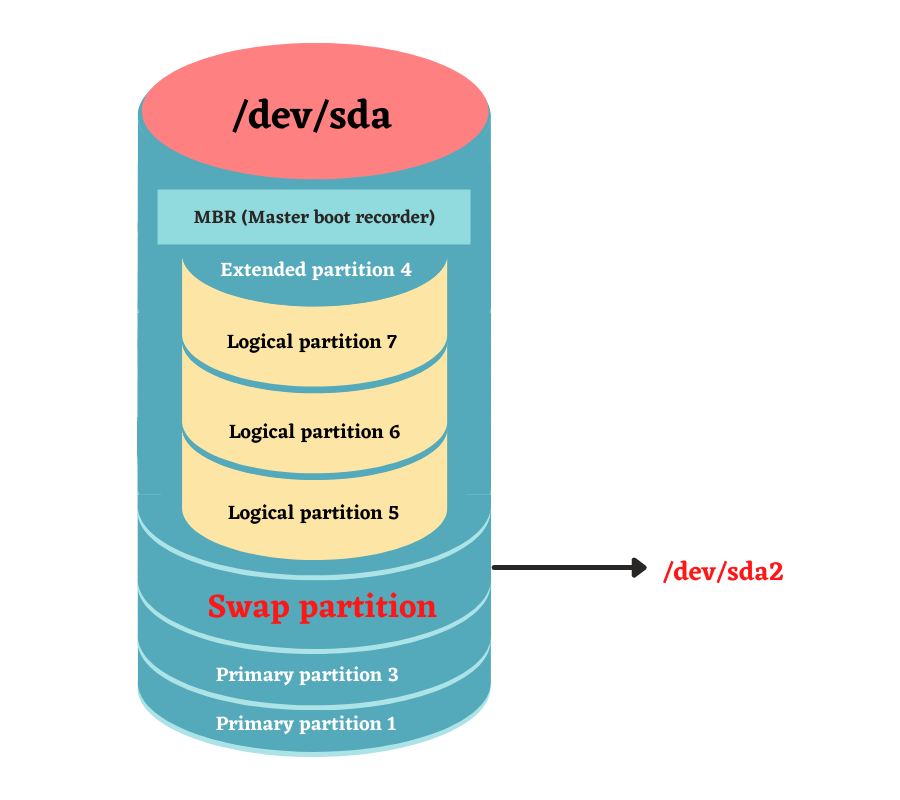
\includegraphics[scale=.5]{content/chapter8/images/swap.png}
			\caption{Swap partitions}
			\label{swap_naming}
		\end{figure}		
		
		\paragraph{Recommended swap partition size}
		
		\begin{tabulary}{1.0\textwidth}{|p{10em}|p{10em}|}
			\toprule
			\textbf{Amount of RAM installed in system} & \textbf{Recommended swap space}\\
			\midrule
			≤ 2GB & 2x RAM \\
			\hline
			2GB – 8GB & = RAM \\
			\hline
			8GB – 64GB & 4G to 0.5x RAM \\
			\hline
			>64GB & Minimum 4GB\\
			\bottomrule
		\end{tabulary}
		
		
	\end{itemize}

\newpage

\paragraph{fdisk command option to create a swap partition}

\begin{itemize}
	\item \textbf{t}: Change type of partition.
\end{itemize}

Eg:
\begin{figure}[h!]
	\centering
	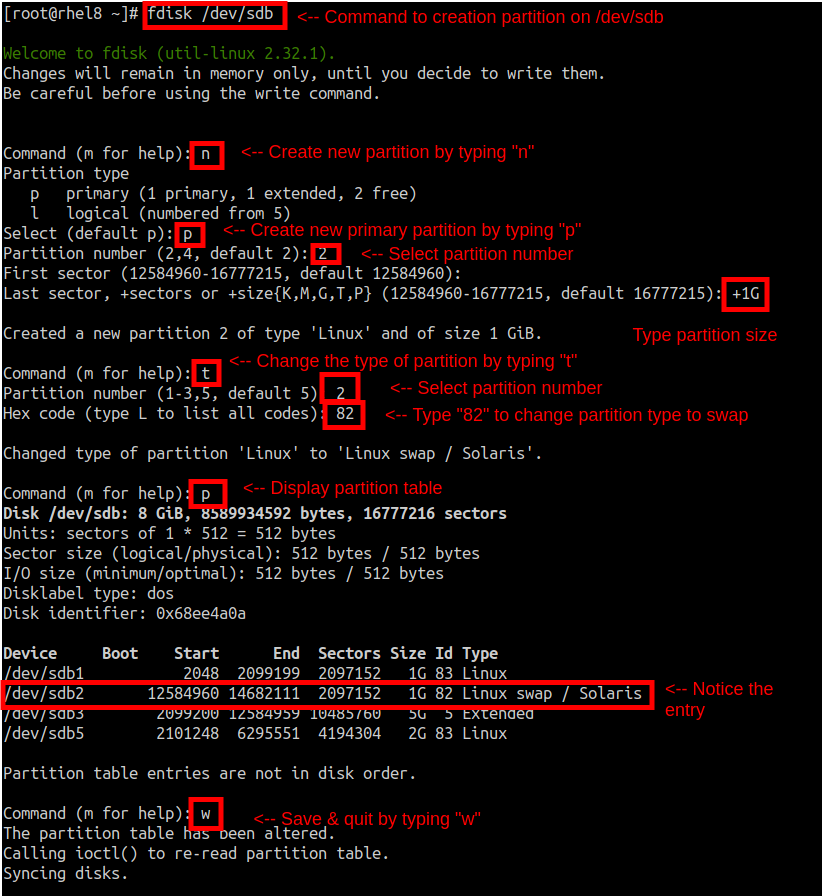
\includegraphics[scale=.4]{content/chapter8/images/swap_part.png}
	\caption{Creating swap partitions}
	\label{primary_swap}
\end{figure}		

	
\end{flushleft}

\newpage

